\scanpage{18}
\mspage{16}

Le théorème de Thom est alors qu'un $x\in H^{\bullet}(X)$ est dans $S(X)$ sss il est
\deleted{\unsure{stable}}\inserted{fixe} par G, i.e. satisfait $A^{+}.\ x=0$. (Pourquoi cette condition est-el\unsure{l}%
le déjà nécessaire ?) Une autre façon de le voir est de dire que le
foncteur $H^{\bullet}$ considéré comme allant de la catégorie $\underline{S}$ précédente dans
la catégorie des \deleted{\unsure{vectoriels}} représentations de G dans des vectoriels
sur $\underline{F}_2$ , est pleinement fidèle. \deleted{Comme G \unsure{est}} Quand on prend l'enveloppe
pseudo-abélienne, on trouve une sous-catégorie pleine de la catégorie des
représentations de G, mais il est douteux qu'on trouve une catégorie abé-%
lienne, voire \unsure{\deleted{t}l|\deleted{l}t}a catégorie de toutes les représentations de G de dimensi\unsure{o|c}
finie sur $\underline{F}_2$ . (Quelle est la structure de G, qui est prolisse; d'après
Quillen, il serait pro-u\unsure{\deleted{i}n|\deleted{n}i}ipotent ....). Ici G bien sûr joue le rôle d'u\unsure{n|r}
groupe de Galois motivique, mais contrairement à la situation familière,
il semble qu'il soit fortement non réductif (et d'ailleurs le corps de
défi\unsure{nit}ion dans tout ceci est $\underline{F}_2$ , et non $\underline{Q}$ ! ).
\margin{\handwritten{ui, car son\\
nneau affine\\
\unsure{t} une \unsure{algèbre}\\
\unsure{y}nômes à une\\
\unsure{f}inité d'indéterminées,\\
\deleted{\illegible{1}} \unsure{réunion d'algèbres de}\\
\unsure{polynômes} à \unsure{augmentation}\\
\unsure{is} stables par $\Delta$}}

Quillen\deleted{t} donne une généralisation de la construction d'une caté-%
gorie universelle $\underline{B}$ au cas où on travaille avec des variétés pas néeessa%
rement propres (mais $f.$ n'étant supposé défini que pour f propre), et
quand on introduit une condition d'orientation \inserted{stable} sur les \uline{morphismes}
\margin{\figure{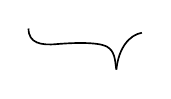
\begin{tikzpicture}[x=.18cm,y=.18cm,line width=.6pt]
\draw (0,1.65) .. controls (0,.6) and (.9,.45) .. (2,.55)
 .. controls (3.8,.7) and (5.35,.65) .. (5.7,.25)
 .. controls (6.15,-.1) and (6.12,-.9) .. (6.2,-1.25);
\draw (6.2,-1.25) .. controls (6.35,.25) and (7.1,1.2) .. (8,1.35);
\end{tikzpicture}}}
envisagés , via un morphisme $H\to BO(\infty)$, où H est un H-espace (commuta%
tif, associatif et unitaire ?): une orientation de $f:X\to Y$ sera un
relèvement homotopique de $X\to BO$, défini par \deleted{$f^{\bullet}(\unsure{T|Y}$} $T_X-f^{\bullet}(T_Y)$ , en $X\rightharpoonup\unsure{H|F}$
les éléments de $H(X,Y)$ seront définis par des diagrammes de morphismes
orientés $Z\to X$, $Z\to Y$, le deuxième étant propre, m\unsure{\deleted{u}o|\deleted{o}u}dulo bords de tels.
En tant qu'ensemble, il se définit aussi en termes de la vari\handwritten{\unsure{é}}té XxY
munie simplement de la famille des supports formée des ensembles fermés
propres sur Y ..... \handwritten{Les $B^H_m(X)$ (X compact \unsure{disons}) peuvent}
\handwritten{se décrire homotopiquement à la Thom, comme les groupes d'homotopie}
\handwritten{stables d'\unsure{espaces} \uline{Hom}$(X,M\unsure{H}(N-m))$ -{}-{}-{}-{}-.}

\handwritten{cf exposé. Karoubi à \begin{tabular}[t]{@{}c@{}}Bourbaki\\[-.8ex]
\begin{tikzpicture}[x=.24cm,y=.24cm,line width=.55pt]
\draw (0,0) .. controls (.2,-.08) and (.55,-.05) .. (.85,-.03);
\draw (1.05,-.02)--(1.65,.1);
\draw (2.05,.02)--(2.95,.04);
\draw (3.75,-.03)--(4.55,0);
\end{tikzpicture}
\end{tabular}}

\margin{17}
